\documentclass[type=normal, year=2014/15]{bdad_exam}
\usepackage[portuguese]{babel}
% Document
\begin{document}
{
\renewcommand{\thechapter}{\arabic{chapter}N}
\setcounter{chapter}{14}
\exam{Exame normal 2014/15}

\question{Pergunta 1} 
No diagrama de classes UML uma classe é:
\begin{enumerate}[label=\alph*.]\itemsep0em
    \item Nenhuma das outras respostas
    \item Um conjunto de objetos relacionados entre si;
    \item Não responder.
    \item Um conjunto de objetos diferenciáveis por serem descritos por conjuntos distintos de atributos;
    \item \textbf{Um descritor de um conjunto de objetos que partilham as mesmas propriedades; \greencheckmark}
\end{enumerate}

\question{Pergunta 2}
Anulada

\question{Pergunta 3}
Diga em que forma normal se encontra o esquema relacional $R(A,B,C,D,E)$ sabendo que contém as seguintes dependências funcionais $DF=\{A \rightarrow C; A,B \rightarrow D,E\}$ e que os 5 atributos são atómicos, i.e., têm domínios singulares?
\begin{enumerate}[label=\alph*.]\itemsep0em
    \item Não responder.
    \item 3ª FN
    \item \textbf{1ª FN \greencheckmark}
    \item BCFN
    \item 2ª FN
\end{enumerate}
A única chave-candidata é $\{A,B\}$.

Para uma relação estar na 2ª FN, tem que garantir que não tem nenhuma dependência funcional em que um atributo não-primo dependa de um subconjunto propriamente dito de uma chave candidata. Os únicos atributos primos são $A$ e $B$, por isso na relação $A \rightarrow C$ temos o atributo não-primo $C$ a depender funcionalmente do conjunto $\{A\}$ que é um subconjunto propriamente dito da chave candidata $\{A,B\}$.

O enunciado garante que todos os atributos são atómicos, logo $R$ está pelo menos na 1ª FN.

\question{Pergunta 4} 
Qual o melhor modo de mapear em LDD-SQL o seguinte diagrama de classes UML?
\begin{center}
    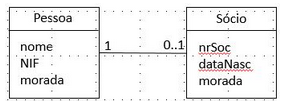
\includegraphics[scale=0.6]{questions/2015N_02.png}
\end{center}
\begin{enumerate}[label=\alph*.]\itemsep0em
    \item - \\
    \begin{lstlisting}[language=SQL]
CREATE TABLE Pessoa (
    idPessoa INTEGER PRIMARY KEY AUTOINCREMENT,
    nome TEXT, NIF TEXT, morada TEXT,
    idSocio INTEGER REFERENCES Socio(idSocio)
);
    \end{lstlisting}
    \item - \\
    \begin{lstlisting}[language=SQL]
CREATE TABLE Pessoa (
    idPessoa INTEGER PRIMARY KEY AUTOINCREMENT,
    nome TEXT, NIF TEXT, morada TEXT,
);
CREATE TABLE Socio (
    idSocio INTEGER PRIMARY KEY AUTOINCREMENT,
    nrSocio INTEGER, dataNasc DATE, morada TEXT
);
    \end{lstlisting}
    \item Não responder.
    \item \textbf{\greencheckmark} \\
    \begin{lstlisting}[language=SQL]
CREATE TABLE Pessoa(
    idPessoa INTEGER PRIMARY KEY AUTOINCREMENT,
    nome TEXT, NIF TEXT, morada TEXT
);
CREATE TABLE Socio (
    idSocio INTEGER PRIMARY KEY AUTOINCREMENT,
    nrSocio INTEEGR, dataNasc DATE, morada TEXT,
    idPessoa INTEGER REFERENCES Pessoa(idPessoa)
);
    \end{lstlisting}
    \item - \\
    \begin{lstlisting}[language=SQL]
CREATE TABLE Pessoa(
    idPessoa INTEGER PRIMARY KEY AUTOINCREMENT,
    nome TEXT, NIF TEXT, morada TEXT,
    idSocio INTEGER REFERENCES Socio(idSocio)
);
CREATE TABLE Socio (
    idSocio INTEGER PRIMARY KEY AUTOINCREMENT,
    nrSocio INTEGER, dataNasc DATE, morada TEXT,
    idPessoa INTEGER REFERENCES Pessoa(idPessoa)
);
    \end{lstlisting}
\end{enumerate}

\newpage
\question{Pergunta 5}
Qual a expressão em álgebra relacional equivalente à seguinte consulta SQL:
\begin{lstlisting}[language=SQL]
SELECT a,b FROM T1 NATURAL JOIN (SELECT * FROM T2 WHERE c='Ola')
\end{lstlisting}
\begin{enumerate}[label=\alph*.]\itemsep0em
    \item Não responder.
    \item $\sigma_{a,b,c}(T1 \naturaljoin T2)$
    \item $\sigma_{a,b}(T1 \naturaljoin \pi_{c='Ola'}(T2))$
    \item \textbf{$\pi_{a,b}(T1 \naturaljoin \sigma_{c='Ola'}(T2))$ \greencheckmark}
    \item $\pi_{c='Ola'}(T1 \naturaljoin \sigma_{a,b}(T2))$
\end{enumerate}

\question{Pergunta 6}
Os triggers do tipo \texttt{INSTEAD OF} são normalmente usados com:
\begin{enumerate}[label=\alph*.]\itemsep0em
    \item \textbf{Vistas \greencheckmark}
    \item Qualquer instrução LMD-SQL
    \item Tabelas
    \item Qualquer instrução LDD-SQL
    \item Não responder.
\end{enumerate}

\question{Pergunta 7}
Nas linguagens PSM um cursor serve para:
\begin{enumerate}[label=\alph*.]\itemsep0em
    \item Integrar código SQL em linguagens hospedeiras
    \item \textbf{Percorrer os tuplos-resultado de uma dada consulta \greencheckmark}
    \item Executar diversas iterações do mesmo código
    \item Não responder.
    \item Otimizar queries
\end{enumerate}

\question{Pergunta 8}
Os sistemas de controlo de concorrência por bloqueios caracterizam-se por:
\begin{enumerate}[label=\alph*.]\itemsep0em
    \item \textbf{Serem menos suscetíveis de abortarem transações que os sistemas baseados em marcas temporais \greencheckmark}
    \item Não ser possível fazer escalonamentos recuperáveis
    \item Não responder.
    \item Não estarem sujeitos à ocorrência de deadlocks
    \item Não estarem sujeitos à ocorrência de livelocks
\end{enumerate}

\question{Pergunta 9}
O teorema CAP diz-nos que é impossível a um sistema distribuído garantir simultaneamente as seguintes características:
\begin{enumerate}[label=\alph*.]\itemsep0em
    \item \textbf{Consistência, disponibilidade e tolerância particional \greencheckmark}
    \item Atomicidade, consistência, isolamento e durabilidade
    \item Consistência, atomicidade e tolerância particional
    \item Não responder.
    \item Consistência, isolamento e durabilidade
\end{enumerate}

\question{Pergunta 10}
O esquema em estrela de um armazém de dados caracteriza-se por:
\begin{enumerate}[label=\alph*.]\itemsep0em
    \item \textbf{Ter uma só tabela de factos cuja chave primária é constituída pelas chaves externas para cada uma das tabelas dimensão do esquema \greencheckmark}
    \item Ter uma ou mais tabelas de factor cujas chaves primárias são constituídas pelas chaves externas para cada uma das tabelas dimensão do esquema
    \item Estar normalizado na 3ª forma normal
    \item Não responder.
    \item Não ter qualquer referência à dimensão tempo
\end{enumerate}

\information{Informação}
Considere o esquema relacional $R(A,B,C,D,E,F)$ com as seguintes dependências funcionais:
\begin{alignat*}{2}
    & A    && \rightarrow B    \\
    & B    && \rightarrow C, D \\
    & A, D && \rightarrow E
\end{alignat*}

\question{Pergunta 11}
Obtenha justificando uma decomposição na 3ª FN.

\ansseparator

Em primeiro lugar, temos que encontrar uma base mínima de $R$, ao remover DFs e atributos redundantes.

Quanto a DFs redundantes:
\begin{itemize}
    \item $\{A\}^+ = \{A\}$ usando as DFs 2 e 3, logo DF1 não é redundante.
    \item $\{B\}^+ = \{B\}$ usando as DFs 1 e 3, logo DF2 não é redundante.
    \item $\{A,D\}^+ = \{A,B,D\}^+ = \{A,B,C,D\}^+ = \{A,B,C,D\}$, usando as DFs 1 e 2, logo DF3 não é redundante.
\end{itemize}
Quanto a atributos redundantes do lado esquerdo:
\begin{itemize}
    \item Removendo $A$ de DF3 tem-se $\{D\}^+ = \{D\}$, logo $A$ não é redundante em DF3.
    \item Removendo $D$ de DF3 tem-se $\{A\}^+ = \{A,B\}^+ = \{A,B,C,D\}$, logo $D$ é redundante em DF3.
\end{itemize}
Assim ficamos com a seguinte base minimal:
\begin{alignat*}{2}
    & A && \rightarrow B, E \\
    & B && \rightarrow C, D
\end{alignat*}

Agora, para cada DF, criamos novas relações:
\begin{alignat*}{2}
    & R_1 (A, B, E) \\
    & R_2 (B, C, D)
\end{alignat*}

Agora vamos testar se alguma das relações $R_1$, $R_2$ é uma superchave de $R$:
\begin{alignat*}{3}
    & \{A, B, E\}^+ &&= \{A, B, C, D, E\}^+ &&= \{A,B,C,D,E\} \\
    & \{B, C, D\}^+ &&= \{B, C, D\}         &&
\end{alignat*}

Como se pode verificar, nenhuma das relações é superchave de $R$, dado que nenhum dos fechos inclui $F$. Por isso é necessário adicionar uma nova relação com uma chave de $R$.

Através das DFs que dispomos, o melhor que conseguimos fazer é, a partir do fecho de $A$, obter $\{A, B, C, D, E\}$, por isso adicionando $F$ conseguimos alcançar todos os atributos ($\{A,F\}^+ = \{A,B,F\}^+ = \{A,B,C,D,F\}^+ = \{A,B,C,D,E,F\}^+ = \{A,B,C,D,E,F\}$), com a garantia absoluta de que $\{A,F\}$ é uma chave dado que nenhum atributo é sozinho superchave de $R$.

Assim, o resultado final da transformação é o seguinte conjunto de relações e dependências funcionais:
\begin{alignat*}{4}
    & R_1 (A, B, E) &&~~~~&& A && \rightarrow B, E\\
    & R_2 (B, C, D) &&~~~~&& B && \rightarrow C, D\\
    & R_5 (A, F)
\end{alignat*}

\question{Pergunta 12}
Verifique se as diferentes relações que obteve na decomposição se encontram na forma normal de Boyce-Codd. Justifique.

\ansseparator

Uma relação $R$ está na forma normal de Boyce-Codd (BCNF) sse, para toda a dependência funcional não-trivial $\overline{A} \rightarrow \overline{B}$, $\overline{A}$ é uma superchave de $R$.
\begin{itemize}
    \item $R_1$: pela DF $A \rightarrow B, E$ é trivial que $A$ é chave (e logo superchave) de $R_1$, logo $R_1$ não viola a BCNF.
    \item $R_2$: pela DF $B \rightarrow C, D$ é trivial que $B$ é chave (e logo superchave) de $R_2$, logo $R_2$ não viola a BCNF.
    \item $R_3$: não possui nenhuma dependência funcional associada, logo trivialmente não viola a BCNF.
\end{itemize}
Assim, as relações obtidas encontram-se na BCNF.

\question{Pergunta 13}
Construa um modelo concetual de dados em UML para armazenar a informação mantida pelo Serviço de Informática de uma Faculdade. Indique todas as restrições que possam ser úteis para a construção da base de dados.

Os responsáveis pela gestão do serviço de informática de uma faculdade pretendem manter informação sobre os equipamentos e salas que gerem, as reservas realizadas por utilizadores, o pessoal técnico do serviço; e os pedidos de apoio técnico. O sistema deve permitir registar os detalhes de cada equipamento, nomeadamente a referência, data de aquisição, fornecedor, tipo, entre outros. Cada equipamento pode estar associado a uma sala. Os equipamentos e salas devem ter um técnico responsável associado.

Os equipamentos podem ser reservados por estudantes ou professores mas as salas apenas podem ser reservadas por professores. Cada reserva tem sempre associado um técnico responsável, bem como uma data de início e uma data de fim. No caso das salas, regista-se a duração da reserva em horas. Os técnicos do serviço estão organizados em unidades, nomeadamente: helpdesk, redes, sistemas e microinformática.

Os pedidos de apoio técnico podem ser solicitados por qualquer utilizador, estudante ou professor, e são posteriormente associados a um técnico para resolução. Relativamente aos pedidos, importa registar a data de colocação do pedido, a data de resolução, o estado (resolvido ou não), os comentários do utilizador que colocou o pedido, e os comentários do técnico.

\ansseparator

TODO

\information{Informação}
Decidiu iniciar o desenvolvimento de um sítio web para armazenamento e partilha de fotografias e criou uma base de dados com o seguinte modelo relacional:

\begin{lstlisting}[numbers=none]
Photo (id, caption, creationDate, uploadDate, user->User)
\end{lstlisting}

As fotografias sâo identificadas com um id. Para cada fotografia guarda-se a legenda, data em que foi tirada, data em que foi introduzida no sistema e o utilizador que a introduziu.

\begin{lstlisting}[numbers=none]
User (id, name)
\end{lstlisting}

Os utilizadores sào identificados por um \texttt{id}. De cada utilizador armazena-se o seu nome.

\begin{lstlisting}[numbers=none]
Likes (user->User, photo->Photo)
\end{lstlisting}

O utilizador identificado com \texttt{user} gosta da fotografia identificada com photo.

\begin{lstlisting}[numbers=none]
AppearsIn (user->User, photo->Photo)
\end{lstlisting}

O utilizador identificado com \texttt{user} surge na fotografia identificada com photo.

\begin{lstlisting}[numbers=none]
Friend (user1->User, user2->User)
\end{lstlisting}

O utilizador identificado com \texttt{user1} é amigo do utilizador identificado com \texttt{user2}. A amizade é recíproca, portanto se a tabela possui o tuplo (245, 888) também possui o (888,245).

A execução das interrogações deve ser feita numa base de dados SQLite criada com as instruções SQL existentes no ficheiro \texttt{photos.sql}.

Deve escrever a interrogação usando SQL. Como as interrogações serão executadas usando SQLite, devem ser compatíveis com a sintaxe SQL suportada pelo SQLite. Antes da execução de cada instrução deve garantir que o SQLite faz a verificação da integridade referencial através da instrução:

\begin{lstlisting}[language=SQL,numbers=none]
PRAGMA foreign_keys = ON;
\end{lstlisting}

Para cada interrogação é apresentada a resposta esperada para a base de dados associada ao ficheiro \texttt{photos.sql}. Esta informação deve ser utilizada para validar a resposta antes de a submeter. Por omissão a saída do SQLite só apresenta colunas com 10 caracteres. O número de caracteres de cada coluna pode ser ajustado utilizando o comando

\begin{lstlisting}[language=SQL,numbers=none]
.width <num caracteres coluna i> <num caracteres coluna 2> ...
\end{lstlisting}

\question{Pergunta 14}
Liste as legendas das fotografias que foram introduzidas pelo Daniel Ramos 2 dias depois de terem sido criadas. Por exemplo, uma fotografia introduzida no dia 6 de junho de 2015 só deve ser devolvida se tiver sido tirada no dia 4 de junho de 2015. [Nota: A interrogação deverá funcionar independentemente do identificador de Daniel Ramos.]
\begin{center} \begin{tabular}{l}
    \textbf{caption} \\ \hline
    Lightning!
\end{tabular} \end{center}
\lstinputlisting[language=SQL]{2015N_14.sql}

\question{Pergunta 15}
Liste o nome dos utilizadores que não introduziram nenhuma fotografia.
\begin{center} \begin{tabular}{l}
    \textbf{name}     \\ \hline
    Catarina Oliveira \\
    Manuel Pinto      \\
    Jorge Rodrigues   \\
    Miguel Ferreira   \\
    Nuno Reis         \\
    Pedro Ponte       \\
    Augusto Cortez
\end{tabular} \end{center}
\lstinputlisting[language=SQL]{2015N_15.sql}

\question{Pergunta 16}
Qual a média de utilizadores que aparecem nas fotografias que têm mais de 3 pessoas a gostar delas.
\begin{center} \begin{tabular}{l}
    \textbf{Média}     \\ \hline
    2.66667
\end{tabular} \end{center}
\lstinputlisting[language=SQL]{2015N_16.sql}

\question{Pergunta 17}
Liste a legenda das fotografias em que surge o Daniel Ramos ou amigos do Daniel Ramos ou amigos de amigos do Daniel Ramos.
\begin{center} \begin{tabular}{l}
    \textbf{caption}                 \\ \hline
    Lightning!                       \\
    Misty Mountain Hop               \\
    Milky Way                        \\
    The stillness of the Escalante   \\
    Unfolding                        \\
    dance with me in the morning sun \\
    The Silence of Dusk              \\
    What?
\end{tabular} \end{center}
\lstinputlisting[language=SQL]{2015N_17.sql}

\question{Pergunta 18}
Apague todas as fotografias introduzidas antes de 01 de janeiro de 2010 em que surjam menos de 2 utilizadores.
\lstinputlisting[language=SQL]{2015N_18.sql}

\question{Pergunta 19}
Crie um gatilho para garantir que, sempre que se insere um registo em AppearsIn referindo que um utilizador aparece numa fotografia, esse utilizador gosta dessa fotografia.
\lstinputlisting[language=SQL]{2015N_19.sql}
}
\end{document}
